\chapter*{Capítulo 1 \vspace{0.5cm} \break Fundamentos teóricos}
\setcounter{chapter}{1}
\addcontentsline{toc}{chapter}{Capítulo 1: Fundamentos teóricos}

%%%%%%%%%%%%%%%%%%%%%%%%%%%%%%%%%%%%%%%%

\section{Sistemas de capacitación laboral}
La capacitación laboral es un método aplicado por las empresas para que su personal adquiera nuevos conocimientos profesionales. Por lo general, se produce ante un ascenso o incorporación, aunque no son los únicos motivos. Busca perfeccionar al colaborador en su puesto laboral, en función de las necesidades de su empresa. Es un proceso estructurado con metas bien definidas. Surge en el mundo como respuesta a la necesidad de mejorar permanentemente la calidad y formación de recursos humanos. Lo ideal es que se desarrolle de forma continua, ya que la constante formación del personal deriva en resultados positivos tanto para el grupo de trabajo como para la organización en la que se realiza \cite{Denby2010}.

\subsection{Características de un sistema de capacitación}
Un sistema de capacitación puede ofrecer diferentes aplicaciones en función del modelo de negocio que utilice. Su versatilidad permite adaptarse a las necesidades particulares de cada sector. Sin embargo, según \cite{Paez2022}, la mayoría de las capacitaciones contienen las siguientes características:

\begin{itemize}
\item Son capaces de gestionar los distintos cursos impartidos, la asistencia y la inversión en formación de la empresa
\item Asignan a los empleados que deberán asistir y a los profesionales responsables de analizar sus resultados
\item Detectan las carencias formativas del personal antes de que influyan en el desarrollo del trabajo
\item Clasifican las distintas actividades formativas en base a su categoría y catálogo
\item Registran y consultan el progreso del aprendizaje de los empleados en tiempo real
\end{itemize}

\subsection{Importancia de una buena capacitación}
La capacitación laboral juega un papel primordial para el logro de tareas y proyectos, dado que es el proceso mediante el cual los trabajadores adquieren conocimientos, herramientas, habilidades y actitudes para interactuar de forma correcta y segura en el entorno laboral. Entre los principales beneficios que aporta, según \cite{RogelioE.Martinez2002}, se destacan:

\begin{itemize}
\item Calidad y mejora en el resultado de las tareas
\item Reducción en tiempos de trabajo y supervisión
\item Solución de problemas con diferentes visiones
\item Sensibilización ante nuevos retos
\item Desarrollo ético y motivación del personal
\item Seguridad y autoestima en los trabajadores
\item Mayor especialización
\end{itemize}

\subsection{Proceso de evaluación en una capacitación}
La evaluación de una capacitación no puede depender de un solo instrumento o técnica, ya que de esa forma solo se mide un tipo de aprendizaje. Los criterios para calificar que se designen serán mostrados como porcentajes de valor asociados a cada resultado de las actividades realizadas y a su resultado final. Entre los criterios más comunes que se tienen en cuenta están: la exactitud de la respuesta, el proceso que se siguió para llegar a la misma, la cantidad de intentos necesarios utilizados para hallar la solución y, en algunos casos, el tiempo necesitado para responder \cite{Jacobs2012}.

Una evaluación posee dos propósitos fundamentales: analizar en qué medida se han cumplido los objetivos y proporcionar una reflexión de los que realizaron el entrenamiento en torno a su propio proceso de aprendizaje (metacognición). Analizar el cumplimiento de los objetivos permite detectar posibles fallas en el proceso y poder superarlas en un futuro \cite{Aretio2020}.

A modo de resumen, para obtener una correcta evaluación se deben tener en cuenta tantas herramientas como parámetros influyan.

\subsection{Fases del proceso de evaluación}
Según \cite{Aretio2020}, un proceso de evaluación debe estar integrado por cinco etapas fundamentales (\textsl{Figura \ref{fig:fases-evaluacion}}). Cada una de ellas, va a marcar un conjunto de acciones, que al final se interpretarán como un buen entrenamiento:

\begin{enumerate}
\item \textbf{Recogida de datos}: es la recopilación sistemática de toda la información a lo largo del proceso completo de enseñanza-aprendizaje. Los datos recogidos deben tener concordancia con las metas trazadas, ser suficientes, representativos, relevantes y ponderados, en función del peso otorgado a cada uno de los objetivos. En los sistemas en línea estas posibilidades de registrar evidencias son inmensas.
\item \textbf{Puntuación de las pruebas}: se realiza una vez medidos, de manera cuantitativa o cualitativa, los distintos bloques de información, con las ponderaciones, criterios e indicadores que se hayan establecido. Sirve para medir los resultados obtenidos en el entrenamiento.
\item \textbf{Juicio de valor}: puede hacerse limitándose a criterios de grupo (evaluación normativa), refiriéndose a criterios de superación de objetivos y contenidos (evaluación de criterio), o teniendo en cuenta la personalidad, posibilidades y limitaciones del propio sujeto del aprendizaje (evaluación personalizada).
\item \textbf{Toma de decisiones}: habitualmente denominada calificación, se basa en la decisión a partir del resultado. Trae consigo una serie de consecuencias personales, administrativas, económicas y laborales. La acción resultante influye directamente en el adiestrado.
\item \textbf{Información a los interesados}: es la etapa final, que ha de llegar a diferentes destinatarios, aunque principalmente y de forma adecuada, a los capacitados. Es la confirmación de que concluye el entrenamiento y donde se dan a conocer los resultados obtenidos.
\end{enumerate}

\begin{figure}[h]
\centering
 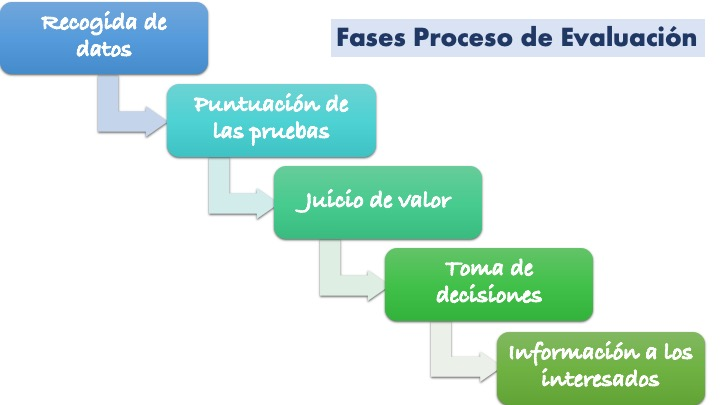
\includegraphics[width=0.6\linewidth]{imagen/fases-proceso-evaluacion.jpg}
 \caption{Fases en un proceso de evaluación.}
 \label{fig:fases-evaluacion} 
\end{figure}

\subsection{Proceso de validación de las respuestas}
Una vez terminada la capacitación se comprueban cuáles de los resultados obtenidos son correctos y cuáles no. Para ello se deben comparar las respuestas del evaluado con una fuente de confianza, que contenga la información verídica de lo que se está tratando. Estas fuentes de confianza se conocen por el nombre de: bases de conocimiento \cite{Rasheed2021}.

A partir de estas bases se verifica si los datos en las respuestas del evaluado coinciden con la información real contenida. Este proceso puede realizarse tanto de manera manual, semiautomática o automática.

%%%%%%%%%%%%%%%%%%%%%%%%%%%%%%%%%%%%%%%%

\section{Sistemas de capacitación automatizados}
Teniendo en cuenta el concepto de capacitación, un sistema de capacitación automatizado es un método de enseñanza alternativo, creado para el adiestramiento de los trabajadores. Es un software que, principalmente, permite el aprendizaje de los usuarios sin necesidad de una supervisión constante. Por lo general, resulta más efectivo que las prácticas de enseñanza presencial, debido a que el estudiante trabaja solo y puede determinar su propia velocidad de aprendizaje, usando una amplia variedad de herramientas y métodos para la transferencia del conocimiento \cite{ISEM2022}.

A modo de resumen, es un programa informático que brinda una solución de recursos humanos, ayuda en la formación de los trabajadores y aumenta la productividad empresarial.

\subsection{Ventajas de un sistema de capacitación automatizado}
Un sistema de entrenamiento asistido por computadora (sistema de capacitación automatizado), permite ofrecer el mismo nivel de adiestramiento para cada usuario del sistema, en cuanto a rigor y evaluación. Uno de los problemas principales de la capacitación de los empleados de manera presencial es que las sesiones son frecuentemente inconsistentes y las diferencias en el nivel de habilidad del formador pueden tener un impacto significativo en el éxito del empleado. Al contar con un sistema automatizado, solo se necesita una base de conocimiento para garantizar el mismo nivel de entrenamiento para todos los capacitados. Por otra parte, una capacitación presencial requiere la existencia de una persona, por lo general un experto, que supervise al adiestrado y califique su rendimiento. En cambio, con un sistema automatizado, no es necesario desempeñar esta tarea, el propio software se encarga de la supervición y evaluación del operario \cite{Kanev2017}.

\subsection{Colores en un sistema de capacitación digital}

\subsection{Tipos de preguntas en un sistema de capacitación automatizado}
A medida que avanza el tiempo se generan nuevos métodos de estudio y con estos, nuevas formas de preguntar y calificar. Sin embargo, a la hora de diseñar un sistema automatizado, no es menos cierto que existen algunas variantes más sencillas y, por ende, más utilizadas. Según \cite{Laguna2016}, los tipos de preguntas que mayormente se emplean en un sistema de capacitación automatizado son:

\begin{itemize}
\item \textbf{Verdadero o falso}: contienen una declaración que se debe indicar si es verdadera o no. Permiten responder en poco tiempo, son fáciles, rápidas de calificar y se corrigen de forma automática.
\item \textbf{Opción múltiple}: se componen de una pregunta (raíz) con múltiples respuestas posibles. Al poder incluir múltiples opciones válidas, podrían darse por superadas al marcar cualquiera de las respuestas o cuando se marquen todas. Se caracterizan por ser fáciles, rápidas de calificar, por corregirse automáticamente y utilizarse para evaluar los conocimientos en una amplia gama de contenidos.
\item \textbf{Emparejar, relacionar u ordenar}: por lo general se emparejan cada una de las opciones del primer bloque con las opciones dadas en el segundo bloque, o se ordenan bloques de modo que quede una secuencia correcta de acuerdo a un patrón previamente establecido. Se suelen usar en aquellos cursos donde la adquisición de conocimientos muy detallados es un objetivo importante. Son preguntas fáciles de diseñar, rápidas de calificar y se corrigen automáticamente. Estadísticamente, se tarda más en responder este tipo de preguntas que las preguntas anteriores.
\item \textbf{Respuesta corta}: basta con que se escriban un par de palabras o una frase sencilla. Una alternativa más común a este tipo de preguntas es la de cubrir los espacios en blanco con una palabra. Son de gran utilidad a la hora de demostrar los conocimientos basados en hechos o palabras claves. La dificultad para calificarlas depende del estilo que se decida emplear.
\end{itemize}

\subsection{Proceso de validación de las respuestas}
En los sistemas de capacitación automatizados pueden utilizarse tres métodos diferentes de validación: manual, semiautomático o automático. Por lo general, el más empleado es el automático, ya que de esta forma se facilita el trabajo para aquellos que deben evaluar a un personal abundante. Según \cite{AltyJames1984}, la manera más efectiva y eficiente de evaluar las respuestas en este tipo de sistemas es mediante el uso de sistemas expertos.